\documentclass[10pt]{article}
\usepackage{../../local}
\urlstyle{same}

\newcommand{\classcode}{Physics 112}
\newcommand{\classname}{Introduction to Statistical and Thermal Physics}
\renewcommand{\maketitle}{%
\hrule height4pt
\large{Eric Du \hfill \classcode}
\newline
\large{HW 09} \Large{\hfill \classname \hfill} \large{\today}
\hrule height4pt \vskip .7em
\small{Header styling inspired by CS 70: \url{https://www.eecs70.org/}}
\normalsize
}
\linespread{1.1}
\begin{document}
	\maketitle
	\section*{Problem 1}
	Let \(  \Phi = E - TS - \mu N\) be the ``grand'' potential
	\begin{enumerate}[label=\alph*)]
		\item Derive the thermodynamic identity \( d\Phi = -S dT - P dV - N d \mu \) 

			\begin{solution}
				Taking inspiration from an earlier homework, we first have:
				\[
				d\Phi = dE - TdS - S dT - \mu dN - N d \mu
				\] 
				And now we use the identity that \( dU = T dS - P dV + \mu dN \). Combining this with the 
				above equation gives us:
				\[
				d\Phi = - S dT - P dV - N d \mu
				\] 
				as desired. 
			\end{solution}
		\item Under what conditions does a system adjust so as to minimize \( \Phi \)?

			\begin{solution}
				The system naturally adjusts itself to minimize \( \Phi \), since entropy increases 
				(by second law)
				so \( \Phi \) decreases as a result. This is also a result that we proved in homework 6. 
			\end{solution}
		\item Suppose you have computed \( \Phi(T, V, \mu) \). How could you use it to determine 
			\( N(T, V, \mu)  \) and \( P(T, V, \mu) \)?

			\begin{solution}
				From the thermodynamic identity, we can get the following relationships:
				\begin{align*}
					-\left( \pdv{\Phi}{\mu} \right)_{T, V} &= N\\
					-\left( \pdv{\Phi}{V} \right)_{T, \mu} &= P
				\end{align*} 
			\end{solution}
		\item Prove that \( \Phi(T, V, \mu) = -kT \ln \mathscr Z\), where \( \mathscr Z = \sum_{\alpha}
			e^{-\beta(E_\alpha - \mu N_\alpha)}\)

			\begin{solution}
				We follow a very similar proof to the one done in section 6.5 proving that \( F = -kT \ln Z \).
				First, we have the thermodynamic identity:
				\[
					\left( \pdv{\Phi}{T} \right)_{V, \mu} = -S
				\] 
				Rearranging for \( S \) in \( \Phi \) gives us:
				\[
					\left( \pdv{\Phi}{T} \right)_{V, \mu} = \frac{\Phi + \mu N - U}{T}
				\] 
				Now, let \( \tilde \Phi = -kT \ln \mathscr Z \). Then, we have:
				\[
					\left( \pdv{\Phi}{T} \right)_{V, \mu} = -k \ln \mathscr Z - kT \pdv{T} \ln \mathscr Z
				\] 
				Focusing in on the second term:
				\begin{align*}
					\pdv{T} \ln \mathscr Z &= \pdv{\beta}{T} \pdv{\beta} \ln \mathscr Z\\
										   &= \frac{1}{kT^2} \frac{1}{\mathscr Z} \pdv{\mathscr Z}{\beta} \\
										   &= \frac{1}{kT^2}\underbrace{\frac{1}{\mathscr Z}
										   \left( \sum_{\alpha}-(E_\alpha - \mu N_\alpha) 
									   e^{-\beta(E_\alpha - \mu N_\alpha)}\right)}_{= -U + \mu N}  
				\end{align*}	
				Therefore, we can now combine these two together:
				\[
					\left( \pdv{\Phi}{T} \right)_{V, \mu} = 
					-k \ln \mathscr Z - kT\left( \frac{U - \mu N}{kT^2} \right) = \frac{\Phi + \mu N - U}{T}
				\] 
				Finally, we show that these two agree at \( T = 0 \). At \( T = 0 \), then 
				\( \Phi = U_0 - \mu N_0\). For the right hand side of this equation, the grand partition
				function at \( T = 0 \) is determined entirely by the leading term so we have:
				\[
				-kT \mathscr Z(0) = -kT \frac{\mu N_0 - U_0}{kT} = U_0 - \mu N_0
				\] 
				Therefore, since these two equations share the same differential equation and also share the 
				same point, they must be equal to each other. 
			\end{solution}
	\end{enumerate}
	\pagebreak
	\section*{Schroeder 7.19}
	Each atom in a chunk of copper contributes one conduction electron. Look up the density and atomic mass 
	of copper, and calculate the Fermi energy, the Fermi temperature, the degeneracy pressure, and the 
	contribution of the degeneracy pressure to the bulk modulus. Is room temperature sufficiently low 
	to treat this system as a degenerate electron gas?

	\begin{solution}
		From Google, we have that the density of copper is 8.96 \( \mathrm{g/cm^3} \), and we know that the 
		formula for the Fermi energy is: 
		\[
		\epsilon_F = \frac{h^2}{8m}\left( \frac{3N}{\pi V} \right)^{2 /3}
		\] 
		Then, consider one mole of copper (this is the only way we get an \( N \) value), so the volume 
		is given by its molar mass divided by the density:
		\[
			V = \frac{m}{\rho} = 7.11 \times 10^{-6} \ \mathrm{m^3}
		\] 
		Therefore, we now throw all the values into Mathematica, and get:
		\[
			\epsilon_F = 1.12 \times  10^{-18} \text{ J}
		\] 
		The Fermi Temperature is given by the equation \( kT = \epsilon_F \), so this gives 
		\[
		T_F = \frac{\epsilon_F}{k} = 85566.2 \text{ K}
		\] 
		Room temperature is \( \sim300 \) K, so this definitely means that room temperature is low enough 
		for the system to be treated as a degenerate gas. The Pressure is given by the equation 
		\[
			P = \frac{2N\epsilon_F}{5V} = 3.819 \times 10^{10} \  \mathrm{N / m^2}
		\] 
		Then, since we have \( P = \frac{2}{3}\frac{U}{V} \) and \( B = \frac{10}{9} \frac{U}{V} \), then 
		we know that \( B = \frac{15}{9}P \), so:
		\[
		B = \frac{15}{9}P = 6.3 \times 10^{10}
		\] 
	\end{solution}

	\pagebreak
	\section*{Schroeder 7.22}
	Consider a degenerate electron gas in which essentially all of the electrons are highly relativistic 
	\( \epsilon \gg mc^2 \), so that their energies are \( \epsilon = pc \) (where \( p \) is the magnitude 
	of the momentum vector).
	\begin{enumerate}[label=\alph*)]
		\item Modify the derivation given above to show that for a relativistic electron gas at zero temperature,
			the chemical potential (or Fermi energy) is given by \( \mu = hc(3N / 8 \pi V)^{1 / 3} \).

			\begin{solution}
				We're given in the problem statement that \( \epsilon = pc \) and \( p \) is the 
				magnitude of the momentum vector, which suggests that:
				\[
				\epsilon = c\sqrt{p_x^2 + p_y^2 + p_Z^2}  = c\sqrt{\left( \frac{hn_x}{2L} \right) ^2 + 
				\left( \frac{hn_y}{2L} \right) ^2 + \left( \frac{hn_z}{2L} \right)^2} = \frac{ch}{2L}
				\sqrt{n_x^2 + n_y^2 + n_z^2} 
				\] 
				Now, we know that the chemical potential is given by the energy at the surface 
				of this sphere, so:
				\[
				\mu = \epsilon_F = \frac{hcn_{\text{max}}}{2L}
				\] 
				so all that suffices now is to calculate \( n_{\text{max}} \). To do so, we need to calculate 
				the number of occupied states on the surface of the sphere. Because the geometry 
				in this case is the same as in the classical case, the equation doesn't change: 
				\[
				N = \frac{\pi n_{\text{max}}^3}{3} \implies n_{\text{max}} = \left( \frac{3N}{\pi} \right)^{1 /3}
				\] 
				Therefore, we have:
				\[
				\mu = \frac{hc}{2L} \left( \frac{3N}{\pi} \right)^{1/3} = hc\left( \frac{3N}{8\pi V} \right)^{1 / 3}
				\] 
				as desired. 
			\end{solution}
		\item Find a formula for the total energy of this system in terms of \( N \) and \( \mu \).

			\begin{solution}
				The total energy can be calculated straight from \( \epsilon(n) \), where \( n = 
				\sqrt{n_x^2 + n_y^2 + n_z^2} \), using equation 7.41:
				\[
					U = 2 \int_0^{n_{\text{max}}} dn \int_0^{\pi /2}d \theta \int_0^{\pi / 2} d\phi n^2 
					\sin \theta \epsilon(n)
				\] 
				Subsituting \( \epsilon(n) \) into the equation, we get:
				\[
				U = 2 \frac{hc}{2L} \frac{n_{\text{max}}^4}{4} \frac{\pi}{2} = \frac{\pi h c n_{\text{max}}^4}{8L}
				\] 
				Using the fact that \( \pi n_{\text{max}}^3 = 3N \) and \( \mu = \frac{hc n_{\text{max}}}{2L} \), 
				we get: 
				\[
				U = \frac{3}{4}N \mu
				\] 
			\end{solution}
	\end{enumerate}
	\pagebreak
	\section*{Schroeder 7.23}
	A \textbf{white dwarf} star (see Figure 7.12) is essentially a degenerate electron gas, with a bunch of 
	nuclei mixed in to balance the charge and to provide gravitational attraction that holds the start 
	together. In this problem you will derive a relation between the mass and the radius of a white dwarf 
	star, modeling the star as a uniform-density sphere. White dwarf stars tend to be extremely hot by our 
	standards; nevertheless, it is an excellent approximation in this problem to set \( T = 0 \).
	\begin{enumerate}[label=\alph*)]
		\item Use dimensional analysis to argue that the gravitational potential energy of a uniform-density 
			sphere (mass \( M \), radius \( R \) ) must equal 
			\[
				U_{\text{grav}} = -(\text{constant}) \frac{GM^2}{R}
			\] 
			where (constant) is some universal constant. Be sure to explain the minus sign. The constant
			turns out to equal 3/5; you can derive it by calculating the (negative) work needed to 
			assemble the sphere, shell by shell, from the inside out.

			\begin{solution}
				I'm not really sure what this problem is asking exactly. The units of \( G \) is 
				\( \mathrm{m^3 kg^{-1} s^{-2}} \), so the right hand side has units of 
				\( \text{kg m} / \mathrm{s^2} \), which is precisely the units of energy. We're also asked to 
				calculate the prefactor itself, so to do that, recall the classical formula for the gravitational
				potential of an object:
				\[
				U = -\frac{GMm}{R} \longrightarrow dU = -\frac{GM}{R} dm
				\] 
				Now, we integrate this from \( 0 \) to \( M \) :
				\[
				U = \int_0^M -\frac{GM}{R} dm
				\] 
				Now, we will integrate this in shells, so we can express \( M \) and \( dm \) in terms of 
				\( r \). Specifically, for a spherical shell of thickness \( dr \), then we have:
				\( d m = 4\pi r^2 dr \), and \( M = 4 / 3 \pi r^3 \rho\). Therefore, this integral 
				becomes:
				\begin{align*}
					U &= \int_0^M -\frac{G}{r}\left( \frac{4}{3}\pi R^3 \rho \right) (4 \pi r^2 dr) \\
					&= -\frac{16G\pi^2 \rho^2}{3} \int_0^R r^{4} dr	\\
					&= -\frac{16G\pi^2\rho^2}{3}\frac{r^{5}}{5} \\
					&= -G\left( \frac{4}{3}\pi R^3 \rho \right) ^2 \cdot \frac{3}{5R} \\
					&= -\frac{3}{5}\frac{GM^2}{R} 
				\end{align*}
				and the factor of \( 3 /5 \) comes out, as desired. 
			\end{solution}
		\item Assuming that the star contains one proton and one neutron for each electron, and that the 
			electrons are nonrelativistic, show that the total (kinetic) energy of the 
			degenerate electrons equals 
			\[
				U_{\text{kinetic}} = (0.0088) \frac{h^2 M^{5 / 3}}{m_e m_p^{5 / 3}R^2}
			\] 
			The numerical factor can be expressed exactly in terms of \( \pi \) and cube roots 
			and such, but it's not worth it.

			\begin{solution}
				We know that the formula for the kinetic energy is given by:
				\[
				U_{\text{kinetic}} = \frac{3}{5}N \epsilon_F = 
				\frac{3h^2 N}{40 m_e} \left( \frac{3N}{\pi V} \right) ^{2 / 3}
				\] 
				so all that remains now is to figure out \( N \) and \( V \). Because we're modeling the dwarf as 
				a perfect sphere, then we know that \( V = \frac{4}{3}\pi R^3 \). Further, the problem 
				statement says that there is one proton and one neutron for each electron, meaning that 
				here, \( N = M/(m_p + m_n + m_e) \). Then, we take the fact that protons and neutrons
				are approximately equal in mass and the fact that by comparison electrons are negligible 
				mass so we can combine the \( m_p \) and \( m_n \) terms, while dropping the \( m_e \) term, 
				leaving us with \( N = M /2 m_p \). Therefore, we're left with:
				\[
				U_{\text{kinetic}} = \frac{3h^2}{40m_e} \frac{M}{2m_p} \left( \frac{3M}{2\pi m_p \left( \frac{4}{3}\pi R^3 \right)^{3 / 2}} \right) 
				\] 
				Simplifying this with Mathematica we get:
				\[
				U_{\text{kinetic}} = \left(\frac{9 \cdot 3^{1 / 3}}{320 \pi^{4 /3}}\right) \frac{h^2M^{5 / 3}}{m_e m_p^{5 / 3}
				R^2}
				\] 
				And as a sanity check, we can verify that the prefactor here does equal \( 0.0088 \), as 
				desired. 
			\end{solution}
		\item The equilibrium radius of the white dwarf is that which minimizes the total energy 
			\( U_{\text{grav}} + U_\text{kinetic} \). Sketch the total energy as a function of \( R \), 
			and find a formula for the equilibrium radius in terms of the mass. As the mass increases, does 
			the radius increase or decrease? Does this make sense?

			\begin{solution}
				Here we're asked to basically just combine the results of the last two problems, so we 
				have 
				\[
					U = (0.088) \frac{h^2 M^{5 /3}}{m_e m_p^{5/3} R^2} - \frac{3}{5}\frac{GM^2}{R}
				\] 
				Ignoring all the constants, I plotted \( y = \frac{1}{x^2} - \frac{1}{x}  \) on 
				Mathematica, which gives the following plot:
				\begin{center}
					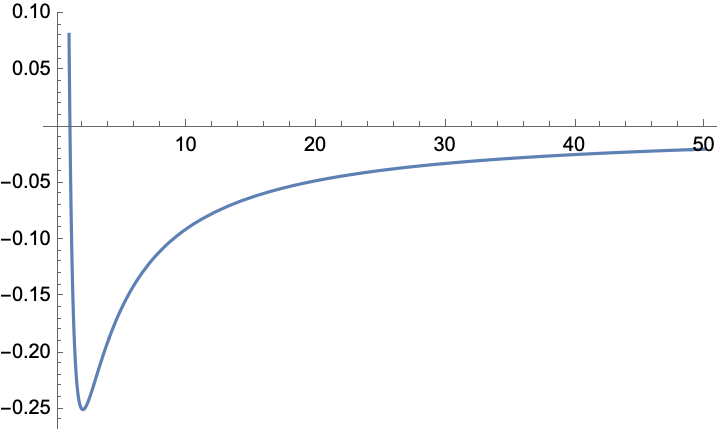
\includegraphics{q3c.png}
				\end{center}
				To find the equilibrium radius, we have to find when the derivative of \( U \) is 
				equal to zero:
				\[
					0 = \dv{U}{R} = \dv{R} \left( \frac{A}{R^2} - \frac{B}{R}\right) = -\frac{2A}{R^3} + 
					\frac{B}{R^2}
				\] 
				Solving for \( R \), we get:
				\[
					R = \frac{2A}{B} = 2\frac{\frac{(0.0088)h^2M^{5 /3}}{m_e m_p^{5/3}} }
					{\frac{3}{5}GM^2} \propto \frac{1}{M^{1/3}}
				\] 
				%update this description
				This means that the equilibrium radius decreases as \( M \) increases. This makes sense, 
				as increasing the mass makes the gravitational potential term dominate, meaning that there is 
				less kinetic energy available, hence giving us a smaller radius.  
			\end{solution}
		\item Evaluate the equilibrium radius for \( M = 2 \times 10^{30} \) kg, the mass of the sun. Also 
			evaluate the density. How does the density compare to that of water?

			\begin{solution}
				Throwing all these values into Mathematica, we get:
				\[
				R = 7.16 \times 10^{6} \text{ m}
				\] 
				This is surprisingly close to the actual value for the radius of the sun! 
				The density is the mass divided by the volume, so we have:
				\[
					\rho = 1.29 \times 10^{9} \ \mathrm{kg/m^3}
				\] 
				this is way more dense than water, I'm not sure what else this question was trying to get me 
				to say.
			\end{solution}
		\item Calculate the Fermi energy and the Fermi temperature, for the case considered in part (d). Discuss
			whether the approximation \( T = 0 \) is valid. 

			\begin{solution}
				The Fermi energy is given by 
				\[
				\epsilon_F = \frac{h^2}{8m}\left( \frac{3N}{\pi V} \right)^{2 /3}
				\] 
				and using our earlier formulas for \( N \) and \( V \), this gets us:
				\[
					\epsilon_F = \frac{3^{4 / 3} h^2M^{2 / 3}}{32 m_e m_p^{2/ 3} R^2 \pi^{4 /3}}
				\] 
				Now, throwing all these values into Mathematica we get:
				\[
				\epsilon_F = 3.1149 \times  10^{-14} \ \text{J}
				\] 
				Then, dividing this by the Boltzmann constant to find the Fermi temperature:
				\[
				T_F = 2.396 \times 10^{9} \ \text{K}
				\] 
				Even the core of the sun only reaches up to tens of millions of Kelvin, whereas this 
				is on the order of billions of Kelvin. Therefore, our approximation of \( T =0 \) is 
				valid, given how far off we are from the Fermi temperature. 
			\end{solution}
		\item Suppose instead that the electrons in the white dwarf are highly relativistic. Using the result 
			from the previous problem, show that the total kinetic energy of the electrons is now 
			proportional to \( 1 / R \) instead of \( 1 / R^2 \). Argue that there is no stable 
			equilibrium radius for such a star.

			\begin{solution}
				With this consideration, total kinetic energy of a star becomes:
				\[
				U = \frac{3}{4}N \mu = \frac{3}{4}N\epsilon_F 
				\] 
				Plugging this into Mathematica, we get: 
				\[
				U = \frac{3hc}{32}\left( \frac{3}{\pi} \right) ^{ 2/ 3}\left( \frac{M}{m_p} \right) ^{4 / 3}\frac{1}{R} \propto \frac{1}{R}
				\] 
				Therefore, our formula for the total energy will be of the form: 
				\[
				U = \frac{A}{R} - \frac{B}{R} = \frac{A-B}{R} \propto \frac{1}{R}
				\] 
				This function never has a global minimum (or local, for that matter), 
				so we never have a stable point. Hence, a relativistic white dwarf is never stable
			\end{solution}
		\item The transition from the nonrelativistic regime to the ultrarelativistic regime occurs 
			approximately where the average kinetic energy of an electron is equal to its rest energy, 
			\( mc^2 \). Is the nonrelativistic approximation valid for a one-solar-mass white dwarf? Above
			what mass would you expect a white dwarf to become relativistic and hence unstable?

			\begin{solution}
				We know that the average kinetic energy of an electron is:
				\[
				E_{\text{avg}} = \frac{3}{5}\epsilon_F
				\] 
				For a stellar mass white dwarf, the average kinetic energy is \( 1.86 \times 10^{-14} \) J 
				whereas \( m_e c^2 = 8.19 \times 10^{-14}\), meaning that it should be stable. To find the 
				critical mass above which we expect a collapse, we basically have to solve the equation:
				\begin{equation}\label{crit}
				\frac{3}{5}\epsilon_F(M) = m_e c^2
			\end{equation} 
				We have the equation for \( \epsilon_F \) :
				\[
					\epsilon_F = \frac{3^{4 / 3} h^2M^{2 / 3}}{32 m_e m_p^{2/ 3} R^2 \pi^{4 /3}}
				\] 
				and we also know the radius \( R \) as a function of mass, from part (c):
				\[
				R = \frac{2\left( \frac{(0.0088)h^2M^{5 / 3}}{m_em_p^{5 / 3}} \right) }{3 / 5GM^2}
				\] 
				Plugging this value of \( R \) back into \( \epsilon_F \) (you couldn't pay me enough to do this 
				algebra by hand) and solving equation \ref{crit} gives us:
				\[
				M = 6.062 \times 10^{30} \text{ kg}
				\] 
				So any mass above this will collapse, and for reference this is roughly three solar masses.   
			\end{solution}
	\end{enumerate}

	\pagebreak
	\section*{Schroeder 7.25}
	Use the results of this section to estimate the contribution of conduction electrons to the heat capacity 
	of one mole of copper at room temperature. How does this contribution compare to that of 
	lattice vibrations, assuming that these are not frozen out? (The electronic contribution has been measured
	at low temperatures, and turns out to be about 40\% more than predicted by the free electron model 
	used here.) 

	\begin{solution}
		We have the equation for the heat capacity of conduction electrons:
		\[
			C_V = \frac{\pi^2Nk^2T}{2\epsilon_F}
		\] 
		From problem 2 we calculated the Fermi energy to be  \( 5.3 \times 10^{10} \) J, so we now we plug 
		everything in, using \( T = 300 K\) and \( N = N_A \) since that's the quantity of particles we used to
		calculate the Fermi energy in problem 2:
		\[
			C_{V, \text{conduction}} = 0.15154
		\] 
		For the vibrations, we're given that each copper ion has heat capacity \( 3 /2 k_B \), so if we multiply
		this by Avogadro's number:
		\[
			C_{V, \text{vibration}} = 2\left(\frac{3}{2}N k_B\right) = 24.928
		\] 
		So we find that the contribution to the heat capacity from the conduction electrons is relatively 
		negligible compared to the vibrations.
	\end{solution}
\end{document}
